
\documentclass[parskip]{cs4rep}

\usepackage{graphicx}
\usepackage{float}

\begin{document}

\title{AV Assignment 3}

\author{Andrew Burnie & Murray Settle}

%\degree{Artificial Intelligence and Computer Science}

%\project{4th Year Project Report}

\date{\today}

\abstract{This report details the work done and algorithms used in the creation of a Matlab program that would manipulate data taken from a Kinect Sensor as instructed inthe third assignment for the Advanced Vision course at Edinburgh University}

\maketitle

\tableofcontents

%\pagenumbering{arabic}


\chapter{Introduction}

We have been given the task of processing data taken from a Kinect \cite{Kinect} sensor and using this to make changes to the video. In the 36 frame video a man is shown walking past a wall holding a black leaverarch folder in his swinging arm as he walks. This video is to be adapted firstly to change the bakground the man walks across to an image of a field of poppies. This given image would be placed within the section of wall shown in red in figure~\ref{intro1}. The second adaptation is to place a video, of our choice, within the bounds of the folder the man is carrying in each frame so that video plays as he walks. For that reason we have chosen a video called Dramatic Chipmunk, frames in figure~\ref{intro2}.

\begin{figure}[H]
\centering
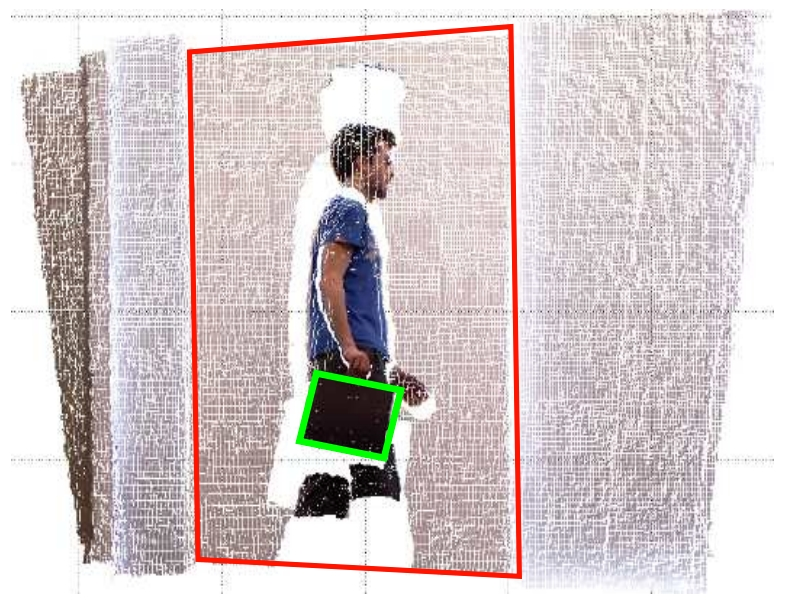
\includegraphics[width=3.5in]{IntroImage1.jpg}
\caption{Section of wall highlighted in red}
\label{intro1}
\end{figure}

\begin{figure}[H]
\centering
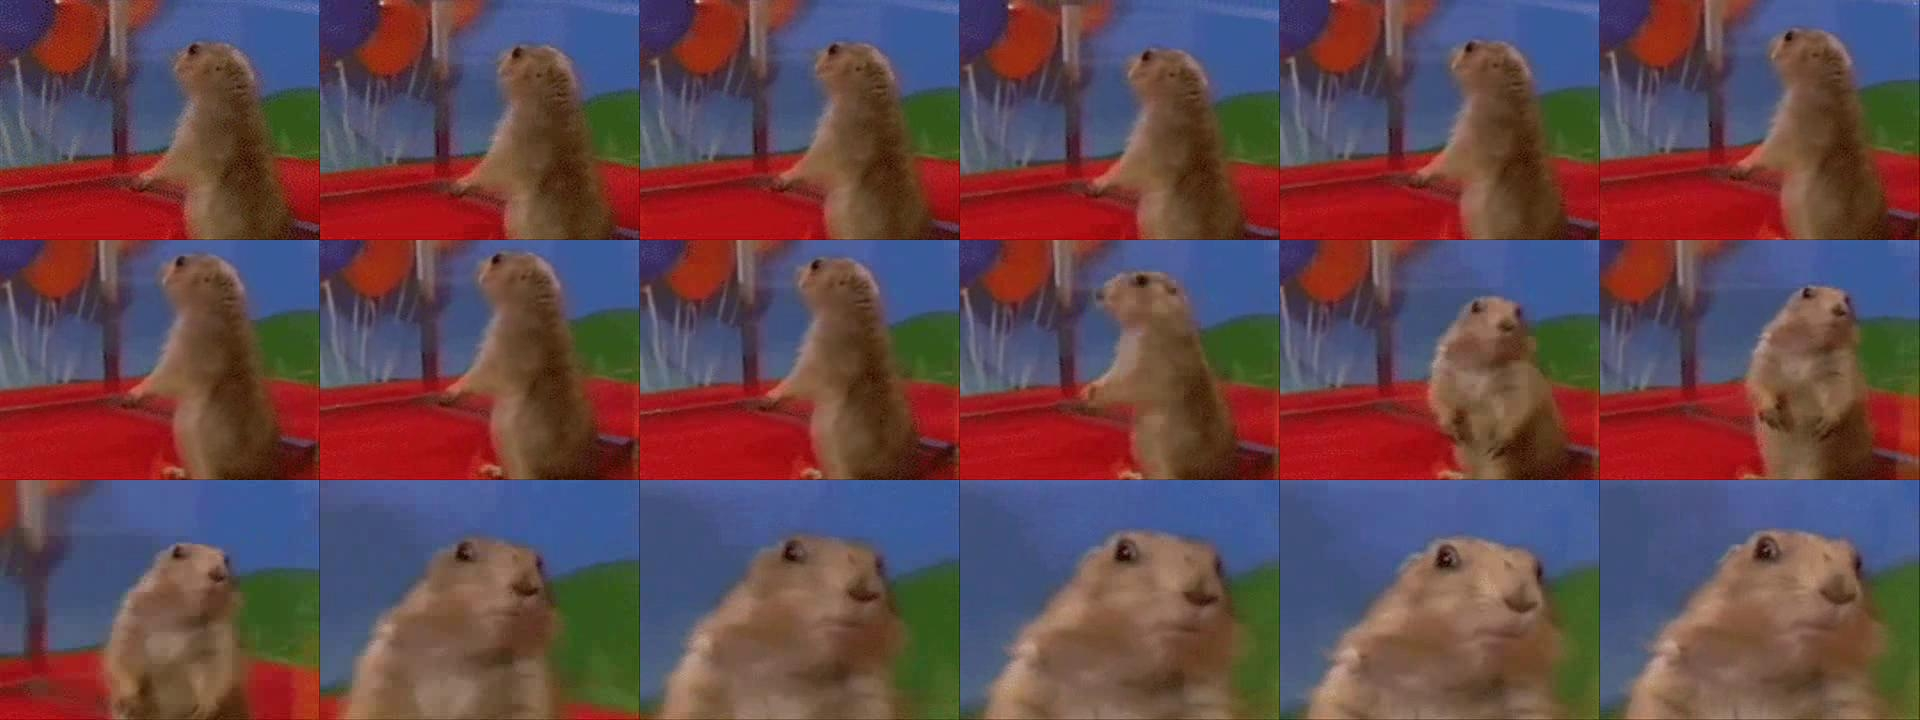
\includegraphics[width=4.5in]{IntroImage2.jpg}
\caption{Dramatic Chipmunk frames}
\label{intro2}
\end{figure}

\section{Data Structure Modification}

\chapter{Extracting the Man}

Background subtraction using depth data

\chapter{Overlaying the Field Image}

\chapter{Extracting the Black Quadrilateral}

Background subtraction using depth data

\chapter{Overlaying the Black Quadrilateral}

\section{Corner Finding}

\begin{enumerate}
\item
Find leftmost point A
\item
Find rightmost point B
\item
Split points into the line from A to B and the line from B to A (using the ordering obtained by boundary tracking)
\item
For each line
    \begin{enumerate}
    \item
    Find straight line between endpoints X and Y
    \item
    Find point Z in the set of points which is furthest from the straight line by distance d (in pixels)
    \item
    If d is less than a threshold, add this line
    \item
    Else, split the set of points into the points between X and Z and the points from Z to Y and recursively perform this line splitting algorithm on those new lines
    \end{enumerate}
\item
For each line, calculate and store its gradient
\item
For each set of 2 lines that share an endpoint
    \begin{enumerate}
    \item
    Decide if gradients of lines are similar
    \item
    If they are, merge them by replacing both lines with a line from the endpoints the lines did not have in common, recalculate the gradient for this line, and go back to 6, and recurse through all lines again
    \end{enumerate}
\end{enumerate}

\chapter{Conclusion}

\chapter{Inclusion of Code}

%\bibliographystyle{plain}

\begin{thebibliography}{50}
\bibitem{Kinect}
Kinect website. http://www.xbox.com/en-US/kinect
\end{thebibliography}

\end{document}

